\section{Dense perception: semantic segmentation and single-image depth}\label{sec:segdepth}
Sections~2--5 used sparse cues (light blobs, optical-flow statistics). This section adds two dense perception tasks on the same clip: \emph{semantic segmentation} (classifying every pixel as road, sidewalk, building/vegetation, sky or dynamic object) and \emph{depth from a single camera}. It is built to be honest about what is possible without pretrained networks.

\subsection{Setting and constraints}
The workspace has no deep-learning framework (no PyTorch or TensorFlow), no pretrained weights and no package installation. A U-Net~\cite{unet} was therefore written from scratch in NumPy with manual back-propagation (\texttt{code/segdepth/unet\_np.py}). It has 96{,}782 parameters (encoder 8--16--32, bottleneck 48, decoder with concatenated skip connections, two $1\times1$ heads), runs on $128\times72$ inputs, and its analytic gradients were checked against finite differences layer by layer. This is a deliberately small model; it is not comparable to published U-Net or SegNet~\cite{segnet} results and it was trained on very little data.

\subsection{Data}
\paragraph{Segmentation labels (hand-made).} I annotated 24 frames spread across the driving portion (one every 7--9\,s) with polygons and boxes on gridded $320\times180$ images: road, sidewalk/roadside ground, building/vegetation (the default fill), sky and dynamic objects (vehicles, riders, pedestrians, animals); the bonnet is ignored. These are \emph{approximate} labels made by the assistant, not expert ground truth: dynamic objects are rectangles, sky at night is subjective, and boundaries are coarse. Sixteen frames are used for training and eight (every third, $t=71,97,124,150,176,201,226,245$\,s) for testing. Sky covers only 3\% of labelled pixels and sidewalk 4\%.

\paragraph{Depth labels (self-supervised from motion).} For 981 frames the ego vehicle's forward translation provides a depth cue: after removing rotation, a static point at depth $Z$ and distance $r$ from the focus of expansion moves radially by $u$ with $Z=\Delta z\,(1+r/u)$, where $\Delta z$ is the distance travelled between two frames 0.133\,s apart (ego speed from Section~2, assumed metric scale). Pixels are kept only with enough parallax, a flow direction consistent with the radial model, texture, and $3<Z<70$\,m, giving $41\%$ valid pixels. These labels are noisy, invalid on moving objects and near the focus of expansion (the black holes in Figure~\ref{fig:depthq}), and their metric scale rests on the same assumed field of view and camera height as before.

\paragraph{Splits.} Depth test frames are three 20\,s blocks of the drive (295 frames, 1.13 million valid pixels); training frames lie at least 3\,s from any test block and from any segmentation test frame (448 frames). The single-image depth task is therefore: given \emph{one} frame, predict what the motion-parallax pipeline would have recovered from \emph{two}, on parts of the drive the model never saw.

\subsection{Training}
One network, two heads, trained alternately for 1{,}800 iterations of each task (batch 8, Adam with cosine decay, about 30\,min on CPU): class-weighted cross-entropy for segmentation; Huber loss on log-depth over valid pixels. Segmentation uses flips, scale-crop and photometric jitter; depth uses only flips and photometric jitter, because scale-cropping changes the geometry the depth head must learn. (A first run that applied scale-crop to depth gave worse segmentation and depth, 0.401 mIoU and 0.470 AbsRel; it is not used.)

\subsection{Segmentation results}
\begin{table}[H]\centering\footnotesize
\resizebox{\linewidth}{!}{\begin{tabular}{lrrrrrrr}
\toprule
Method & Pixel acc. & road & sidewalk & building/veg. & sky & dynamic & mIoU [95\% CI] \\
\midrule
Position prior & 75.9 & 77.1 & 19.3 & 72.7 & 0.0 & 10.8 & 36.0 [33.1,39.1] \\
Gradient boosting (per pixel) & 76.7 & 76.1 & 14.4 & 72.5 & 11.5 & 30.2 & 40.9 [36.7,45.3] \\
U-Net (NumPy, ours) & 79.5 & 78.4 & 17.9 & 73.5 & 33.3 & 42.4 & 49.1 [40.7,57.4] \\
\bottomrule
\end{tabular}
}
\caption{Segmentation on the 8 held-out frames (IoU in \% per class; mIoU 95\% bootstrap CI over frames). Baselines: the per-pixel position prior from the 16 training masks, and gradient boosting on 11 colour, texture and position features per pixel.}\label{tab:seg}\end{table}
The U-Net has the highest pixel accuracy (79.5\% against 76.7\% and 75.9\%) and mIoU (49.1\% against 40.9\% and 36.0\%), driven by the two classes that need appearance rather than layout: dynamic objects (42.4\% IoU against 30.2\% and 10.8\%) and sky (33.3\% against 11.5\% and 0\%). Road and building/vegetation are already captured by the position prior (77.1\% and 72.7\%), and sidewalk is poor for every method (14--19\%; the U-Net's 17.9\% is no better). With only eight test frames the mIoU intervals overlap (U-Net 40.7--57.4\%, gradient boosting 36.7--45.3\%), so the advantage over gradient boosting is suggestive, not established.

\begin{figure}[H]\centering
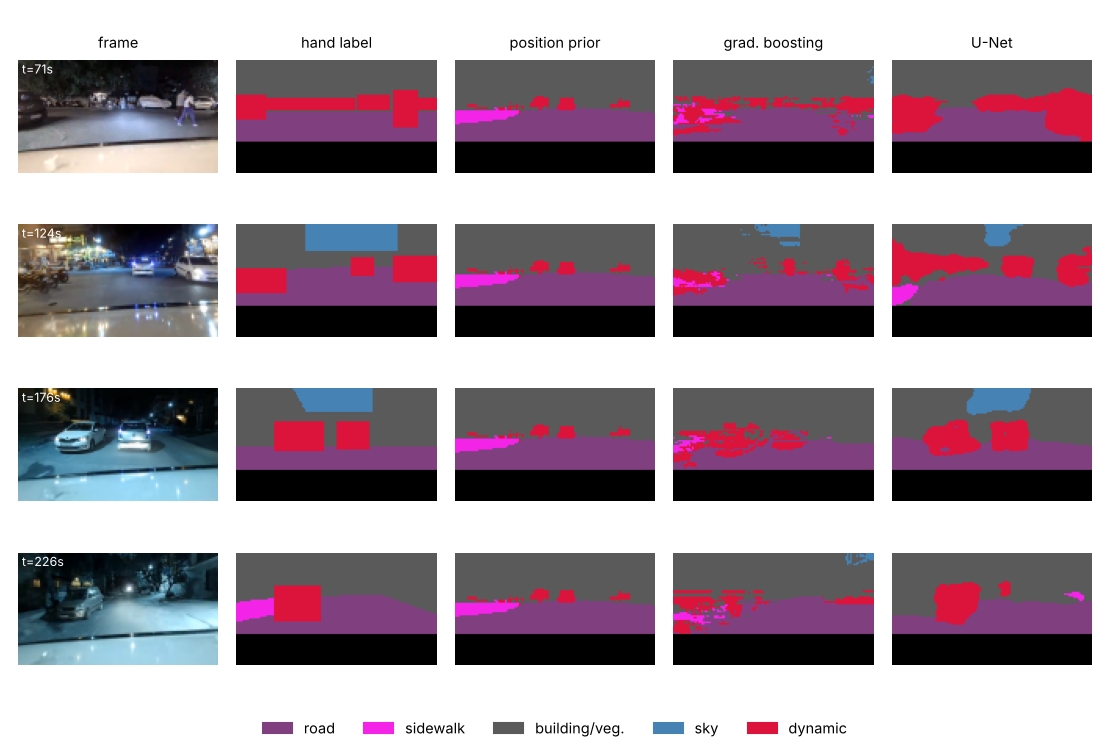
\includegraphics[width=\linewidth]{seg_qualitative.png}
\caption{Four held-out frames: hand label, position prior, gradient boosting and U-Net. The U-Net recovers dynamic blobs and some sky; its dynamic regions are blob-like because the labels are boxes.}\label{fig:segq}
\end{figure}
\begin{figure}[H]\centering
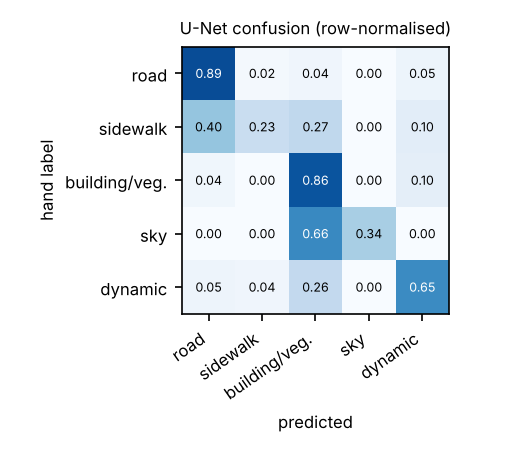
\includegraphics[width=0.48\linewidth]{seg_confusion.png}\hfill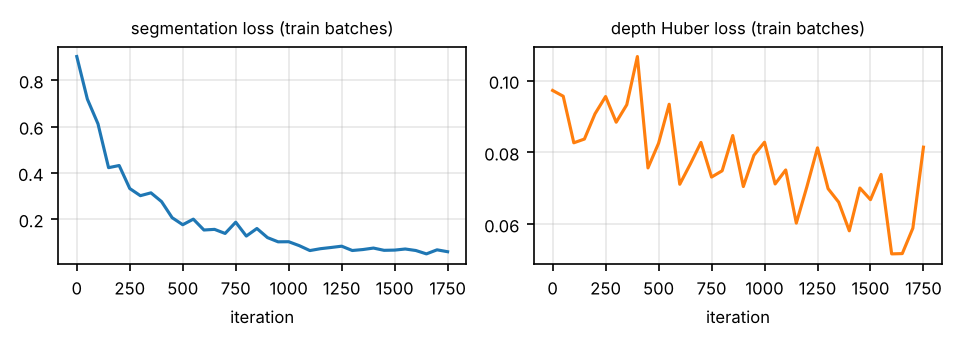
\includegraphics[width=0.5\linewidth]{train_curves.png}
\caption{Left: U-Net confusion matrix on the test frames. Right: training losses (batch values, noisy).}
\end{figure}

\subsection{Single-image depth results}
\begin{table}[H]\centering\footnotesize
\resizebox{\linewidth}{!}{\begin{tabular}{lrrrrrr}
\toprule
Method & AbsRel & RMSE-log & $\delta<1.25$ (\%) & AbsRel (scale-aligned) & SILog & Spearman $\rho$ \\
\midrule
Constant (train median) & 0.502 & 0.557 & 30.3 & 0.425 & 0.557 & -- \\
Row prior & 0.447 & 0.515 & 33.4 & 0.331 & 0.515 & 0.37 \\
Ground-plane geometry & 1.537 & 0.983 & 13.6 & 0.406 & 0.752 & 0.33 \\
Gradient boosting (per pixel) & 0.392 & 0.470 & 38.9 & 0.302 & 0.469 & 0.55 \\
U-Net (NumPy, ours) & 0.442 & 0.511 & 34.6 & 0.350 & 0.511 & 0.46 \\
\bottomrule
\end{tabular}
}
\caption{Depth on the held-out blocks, against the motion-parallax labels (valid pixels only). AbsRel $=\mathrm{mean}|\hat Z-Z|/Z$; ``scale-aligned'' rescales each prediction to the label median. Ground-plane geometry uses $Z=fH/(y-y_h)$ with the assumed $f$ and $H$ applied to every pixel below the horizon.}\label{tab:depth}\end{table}
\begin{table}[H]\centering\footnotesize
\begin{tabular}{lrrrr}
\toprule
Label depth & Valid px & Row prior & Grad. boosting & U-Net \\
\midrule
3--10 m & 101642 & 1.447 & 1.171 & 1.173 \\
10--20 m & 390868 & 0.428 & 0.359 & 0.447 \\
20--35 m & 400427 & 0.197 & 0.228 & 0.269 \\
35--70 m & 233404 & 0.470 & 0.390 & 0.414 \\
\bottomrule
\end{tabular}
\quad\begin{tabular}{lrrr}
\toprule
Predicted class & Valid px & U-Net AbsRel & Ground-plane AbsRel \\
\midrule
road & 183553 & 0.454 & 0.684 \\
sidewalk & 40146 & 0.469 & 1.619 \\
building/veg. & 708135 & 0.444 & 1.686 \\
dynamic & 186023 & 0.419 & 1.816 \\
\bottomrule
\end{tabular}

\caption{Left: AbsRel by label depth. Right: AbsRel by predicted class, U-Net against the ground-plane formula.}\end{table}

The result is modest and should be read as such. The U-Net (AbsRel 0.442) is only marginally better than a row-wise prior that ignores the image (0.447) and is worse than per-pixel gradient boosting (0.392); all three clearly beat a constant (0.502) and the raw ground-plane formula (1.54, which is wrong by a scale factor: scale-aligned it is 0.41; even restricted to pixels the U-Net labels road its AbsRel is 0.68 against 0.45). Per held-out block the U-Net is better than the row prior in only the last block (0.484 against 0.546; 0.408 against 0.374 and 0.438 against 0.427 in the first two). Errors are largest at close range (3--10\,m, AbsRel above 1.1 for every method), where the motion labels are least reliable. In short, the network has learned mostly the scene layout (near ground below, far structure above) and a little appearance; with 448 training frames from one drive and 97k parameters this is expected, and it is not evidence that single-image depth works well in this setting.

\begin{figure}[H]\centering
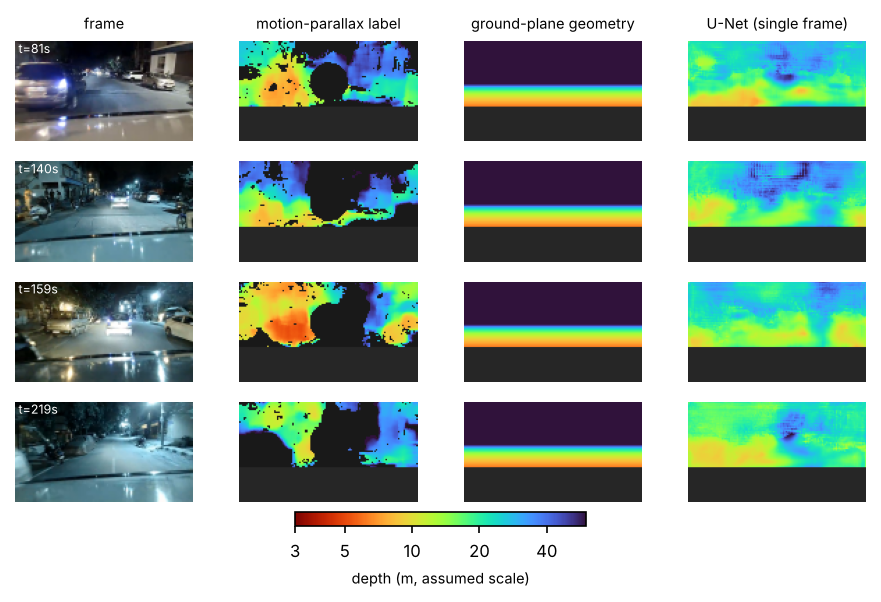
\includegraphics[width=\linewidth]{depth_qualitative.png}
\caption{Four held-out frames: motion-parallax label (black = invalid), ground-plane formula, and U-Net prediction. The U-Net output is smooth and layout-driven.}\label{fig:depthq}
\end{figure}
\begin{figure}[H]\centering
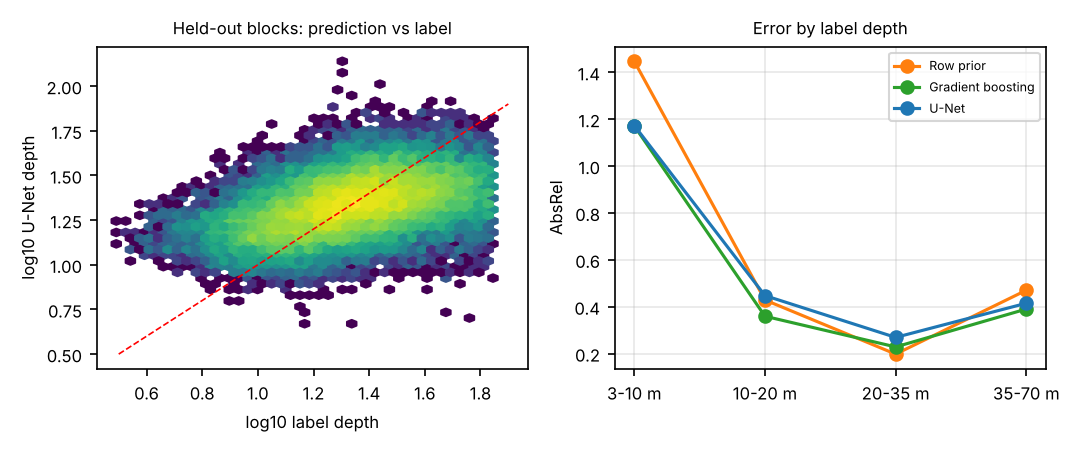
\includegraphics[width=\linewidth]{depth_scatter.png}
\caption{Left: held-out predictions against labels (log scale, density). Right: error by label depth.}
\end{figure}

\paragraph{Cross-check against tail-light ranging.} Fifteen held-out frames contain a detectable tail-light pair, which gives an independent range estimate (1.5\,m lamp spacing, assumed field of view). The U-Net's median depth over the lead vehicle has a median relative error of 0.46, against 0.67 for the row prior, 1.19 for gradient boosting and 1.13 for a constant; its rank correlation with the lamp range is only 0.38 (row prior 0.74). Motion-parallax depth is valid on only 8 of these vehicles and is badly wrong there (median relative error 3.3), which is the expected failure of a static-scene assumption on a moving lead vehicle. With $n=15$ this is anecdotal: it suggests the learned single-frame depth is more useful than motion parallax on moving objects, not that it ranks vehicles reliably.

\begin{figure}[H]\centering
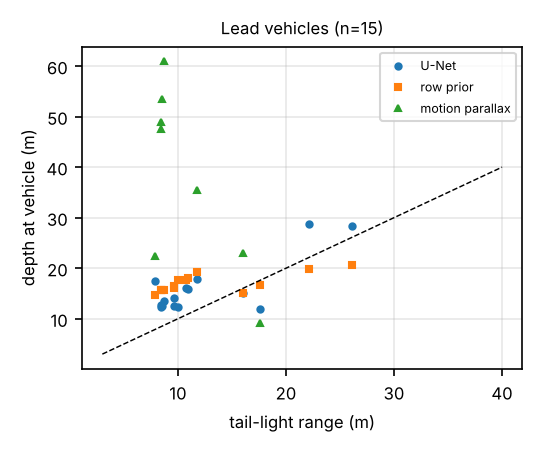
\includegraphics[width=0.5\linewidth]{depth_lamp.png}
\caption{U-Net, row-prior and motion-parallax depth at lead vehicles against tail-light range.}
\end{figure}
\begin{figure}[H]\centering
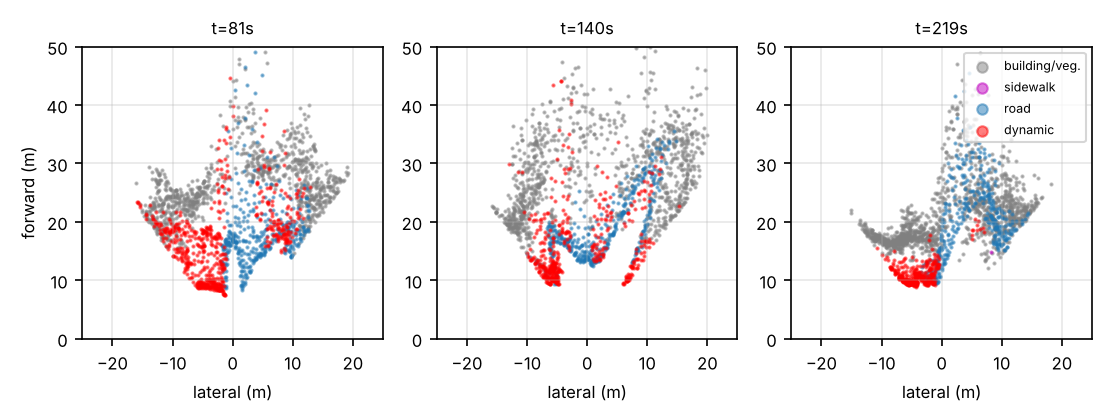
\includegraphics[width=\linewidth]{bev.png}
\caption{Bird's-eye view built from the U-Net depth and segmentation at three held-out times (road blue, dynamic red, building/vegetation grey).}\label{fig:bev}
\end{figure}

\subsection{What the two outputs add: bird's-eye view, road visibility and free-space range}
Combining segmentation and depth gives geometry the planner and the ODD monitor can use. Back-projecting the depth map (Figure~\ref{fig:bev}) gives a coarse bird's-eye view; road pixels trace the drivable corridor and dynamic pixels cluster at 9--15\,m ahead. Running both heads on 973 frames of the drive, two per-frame quantities were computed:
\begin{itemize}\setlength\itemsep{0pt}
\item \textbf{Visible road fraction} in the lower image (mean 0.57; below 0.4 in only 8.7\% of frames), a direct measure of drivable-surface visibility. It is an alternative to the lane-marking proxy of Section~\ref{sec:odd}, which flagged violations 74\% of the time: in this environment drivable surface is mostly visible even though lane markings are not, which supports the argument for ODD attributes that describe the surface rather than the paint.
\item \textbf{Free-space range}, the predicted depth at the far end of the road in the central corridor (median 19.6\,m; 10th percentile 12.5\,m; below 15\,m in 18.5\% of frames and below 15\,m while moving faster than 8\,m/s in 3.8\%).
\end{itemize}
The human driver's speed is positively related to free-space range (Spearman $\rho=0.40$; 95\% block-bootstrap interval 0.21--0.53 over 10\,s blocks) and essentially unrelated to road fraction ($\rho=-0.09$). This is a single drive, both quantities come from imperfect models and the speed is itself an estimate, so it is a descriptive association, not a validated driver model; it does suggest free-space range as a usable input to a speed-adaptation rule.

\begin{figure}[H]\centering
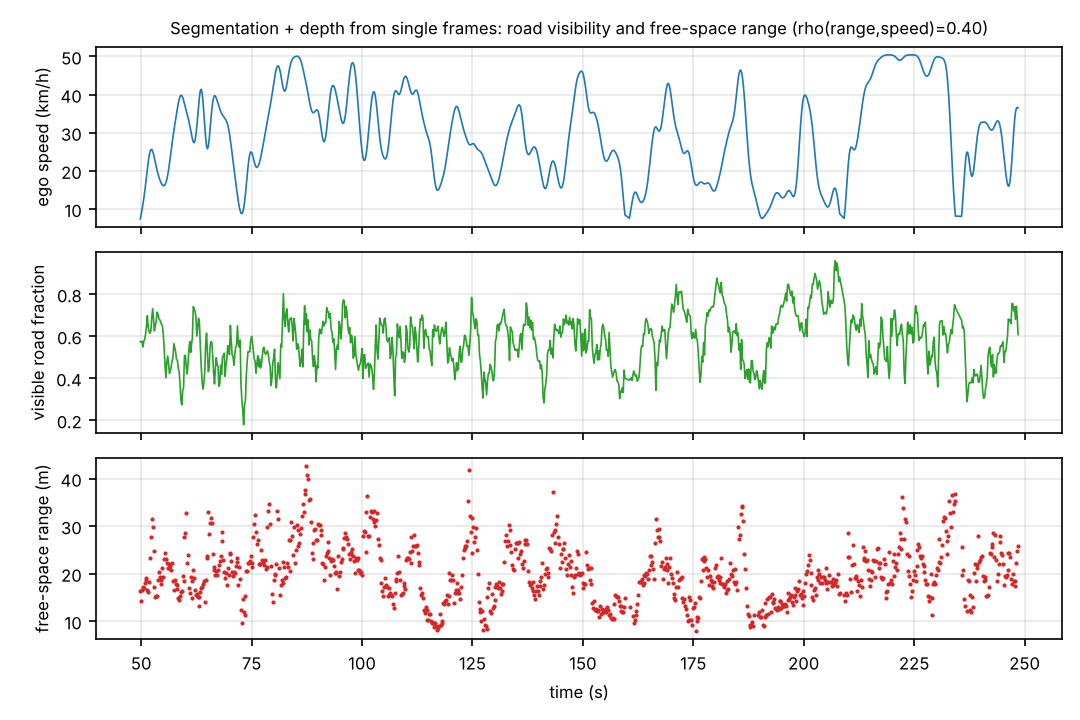
\includegraphics[width=\linewidth]{freespace_timeline.png}
\caption{Speed, visible road fraction and free-space range over the drive, all from single-frame network outputs and the flow-based speed estimate.}
\end{figure}

\subsection{Limitations}
\begin{itemize}\setlength\itemsep{0pt}
\item \textbf{Tiny, single-source data.} Sixteen training and eight test frames for segmentation, one drive for everything; no cross-city or day-time test. Results say nothing about generalisation.
\item \textbf{Approximate labels.} The segmentation labels are my own coarse annotations and the depth labels are noisy motion estimates with an assumed metric scale; the reported scores are measured against these, not against ground truth (no LiDAR or HD-map reference exists for the clip).
\item \textbf{Small custom network.} It is a minimal U-Net, trained for 30 minutes on a CPU; published architectures with pretrained backbones would do far better, and the per-class segmentation and depth numbers here are not comparable to benchmark results.
\item \textbf{Free-space range} depends on the segmentation and depth heads, both weak at long range and near moving objects.
\end{itemize}
